\subsection{Case Study}
Before 2014 the legal procedure of selling a vehicle in Mexico is described in the following
work flow:
\begin{enumerate}
    \item The buyer might check that no legal problems are involved with the vehicle. 
          An online check can be done with the plate number. 
    \item The buyer makes the car payment
    \item The seller endorses his bill to the new owner and gives possession of the car 
    to the buyer.
    %generates an electronic bill for the value of the car and acknowledges payment from the buyer
    \item The change of ownership is notified to the city government. In some cities a 
        change of plates is necessary and a new set of plates is given to the new owner.
\end{enumerate}

From 2014, Mexico joins the paperless culture in the world, so paper bills stopped being 
legal proof of ownership. This led to some problems in the purchase procedure.

With electronic bill, such a work flow provides a vulnerability between steps $2$ and $3$. 
Step $2$ can be generated even without the existence of a physical car. A malicious seller 
could generate multiple apparently original bills and give to multiple buyers before 
they realize the car doesn't exist physically. A certain level of \textit{trust} must 
exist between buyer and seller for the exchange to happen. And this \textit{trust} can be 
maligned. 

This fraud is specially common on car sales between private owners for a couple reasons. 
The first one is the high value of this commodity, which makes it a low risks - high stakes 
trade-off for fraudsters. The other one comes with the definition of car: A portable, efficient, 
and maneuverable transportation vehicle that can be easily removed from the transaction scene 
and hidden afterwards.

Due to the lack of immediate retaliation available to the criminal, he has a time frame where 
the fraud could be repeated multiple times, even if finally, the car exchange takes place with 
an Innocent buyer afterwards.

Currently the solution by dealerships have been to sign officially a physical invoice 
including holograms, stamps, etc. (See Figure~\ref{fig:invoice} for an example). 
However, it fall backs into the loss of paperless culture. We have revised that the case 
study exposed in this section is also active in several countries.
\begin{figure}[hbt]
 %\begin{center}
  \centering
    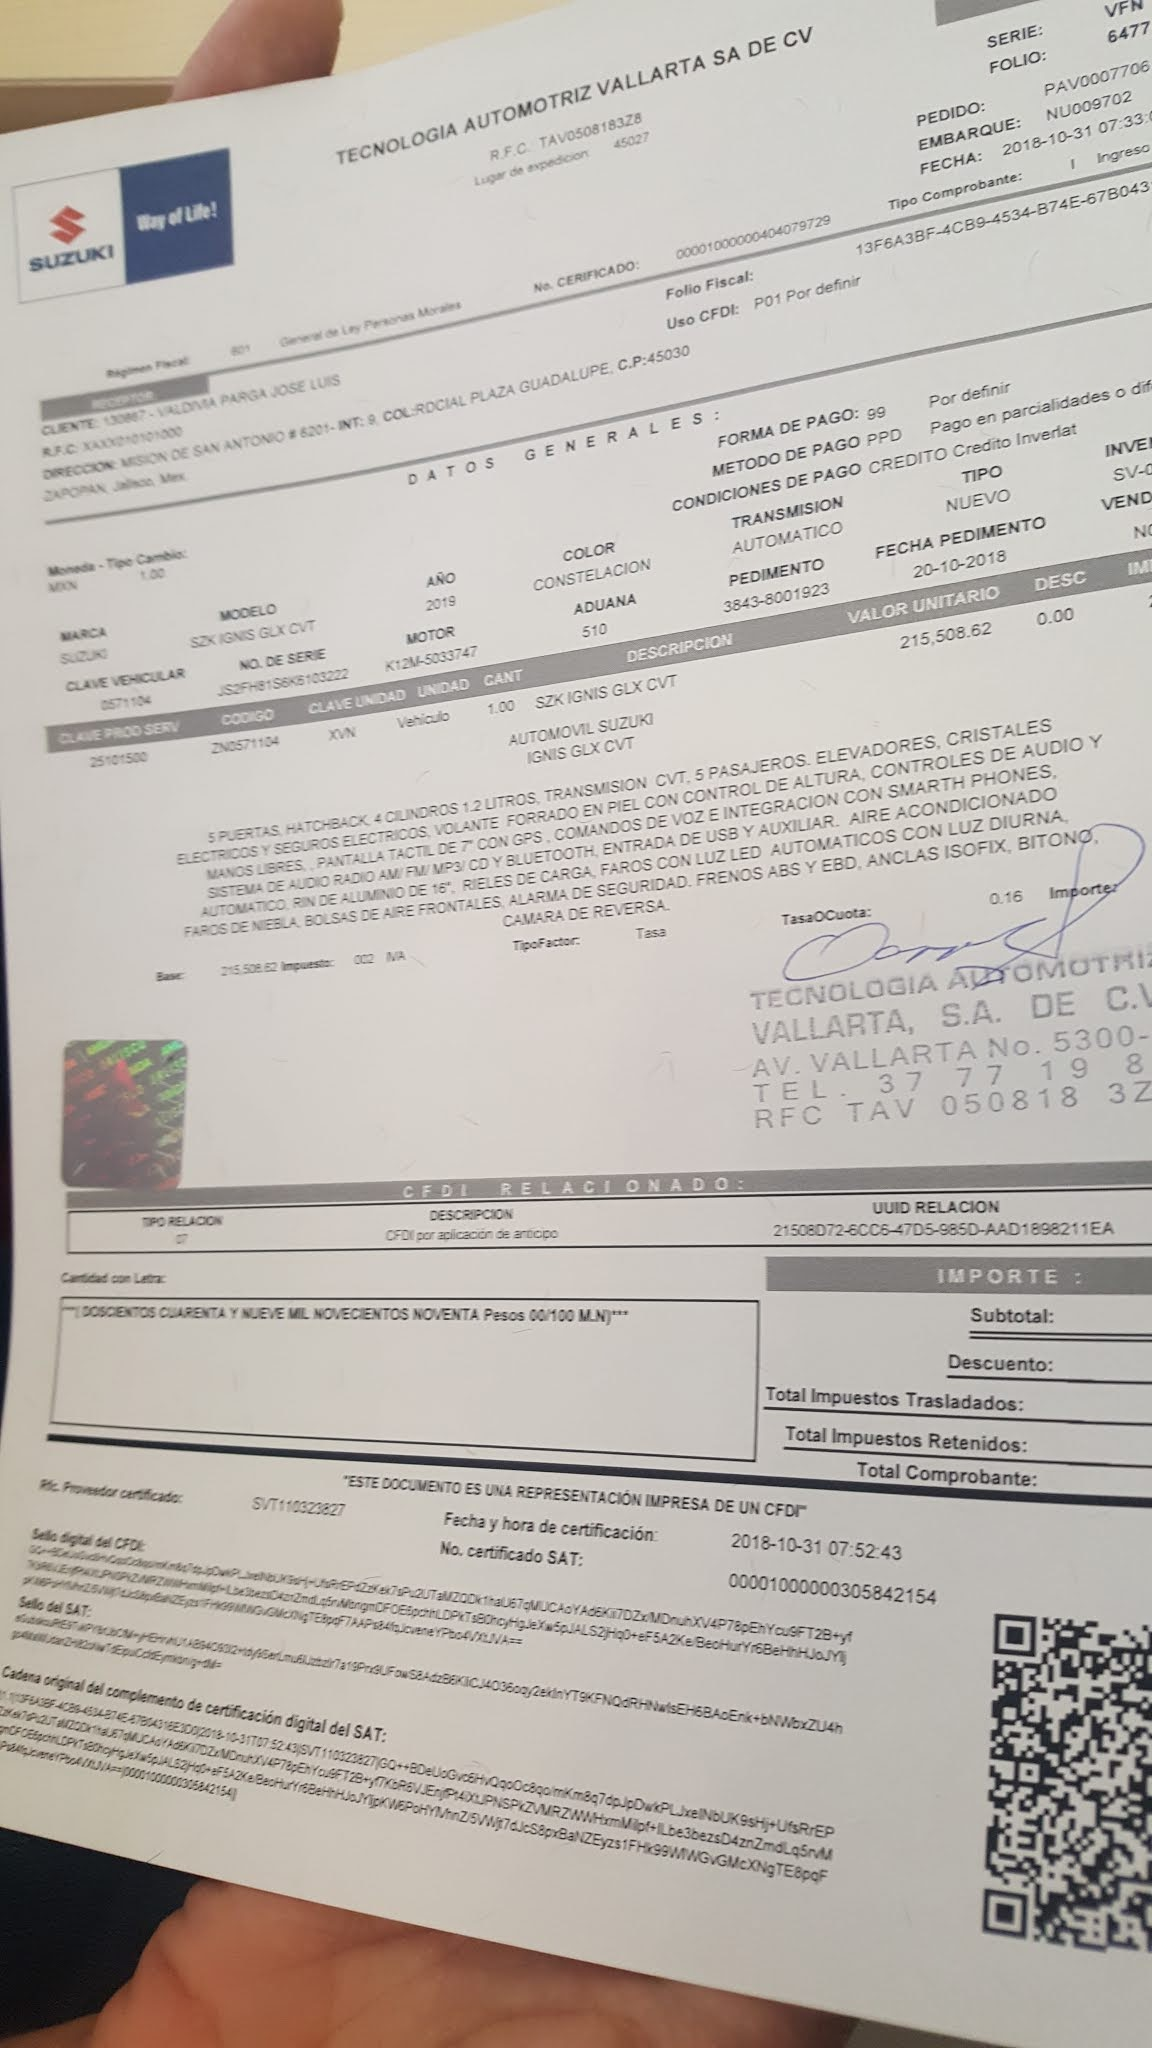
\includegraphics[scale=0.1]{images/invoice.jpg}
        \caption{Formal Invoice including a hologram, a stamp and a signature}
    \label{fig:invoice}
 % \end{center}
\end{figure}

